\documentclass[addpoints]{physlabs}

\labtitle{Conservation of Momentum and Energy}
\labnum{}
\labnumroman{III}
\course{PHYSICS 113 - 121 - 181}
\coursesubtitle{General Physics I and Mechanics}
\date{\today}

\usetikzlibrary{spath3, intersections, patterns, patterns.meta}

\newcolumntype{g}{>{\columncolor{gray!20}}c}

\begin{document}

\maketitle

% PRELAB SECTION
\begin{prelab}

% % \begin{questions}
% %     \begingradingrange{prelab}
%     \question[10] This is the first question
%     \question This the second question
%     \begin{parts}
%         \part[5] This is a part worth 10 marks
%         \part[5] This is a part worth 10 marks
%     \end{parts}
%     \question[5] This the third question
% %     \endgradingrange{prelab}
    
% %     \newcounter{nprelab}
% %     \setcounter{nprelab}{\value{question}}
% % \end{questions}

    \question[1]
    In measurements using the linear track, what is the purpose of measuring the {\bf average fraction lost} for the momentum and energy?
    \begin{solution}[3cm]
    \end{solution}

    \question
    \begin{parts}
        \part[\half] Briefly describe both methods.
        \begin{solution}[3cm]
        \end{solution}
        
        \part[\half] Why might we want to use two independent methods to estimate $v_b$?
        \begin{solution}[3cm]
        \end{solution}
    \end{parts}

\end{prelab}

% LAB SECTION
\begin{labsection}
\begin{objective}
    To experimentally verify the laws of conservation of energy and momentum with two experiments:
    %
    \begin{enumerate}[itemsep=-0.1em]
        \item Testing Newton's First Law and measuring elastic and inelastic collisions using a linear track.
        \item Measuring the velocity of a projectile using a ballistic pendulum and projectile motion.
    \end{enumerate}
\end{objective}

% Theory section
\begin{theory}
    The laws of conservation for momentum and energy are among the most fundamental and useful laws of physics. 
    They aid in the solution of many mechanics problems and come up frequently in many fields of science.

    \subsection*{Newton's Laws, Conservation Laws, and Symmetries}
    
    \textbf{Conservation of momentum} says that if no net force acts on an object of mass $m$, then that object will have constant momentum, $\mathbf{p}$\footnote{Note that momentum is a vector quantity with both magnitude and direction.},
    %
    \begin{equation}\label{eq: momentum}
        \mathbf{p} = m\mathbf{v},
    \end{equation}
    %
    where $\mathbf{v}$ is the object's velocity.
    This is a direct consequence of Newton's second law, which says:
    %
    \begin{equation}\label{eq:newton's second law}
        \mathbf{F}_\text{tot}
        =m\mathbf{a}
        =m\frac{d\mathbf{v}}{dt}
        =\frac{d(m\mathbf{v})}{dt}
        =\frac{d\mathbf{p}}{dt}.
    \end{equation}
    %
    If there is no net force ($\mathbf{F}_\text{tot}=0$) then
    %
    \begin{equation}
        \frac{d\mathbf{p}}{dt}=0 \implies \mathbf{p}=\text{constant}
    \end{equation}
    %
    and momentum is conserved. Conservation of momentum is a restatement of Newton's first law (also known as the \textbf{law of inertia}), which says that an object at rest or in constant-velocity motion will remain in its state of motion unless acted upon by a net external force. Stated in terms of momentum, Newton's second law says that an object's momentum does not change in the absence of some net external force.
    
    \textbf{Conservation of energy} states that the total energy $E$ of an isolated system is neither created nor destroyed; it is transformed between different types. In this experiment, we will be concerned with the conservation (or non-conservation) of kinetic energy, given by
    %
    \begin{equation}\label{eq: kinetic energy}
        K = \frac{1}{2}mv^2.
    \end{equation}

    Conservation laws are intimately related to fundamental \textbf{symmetries}\footnote{The relationship between conservation laws and symmetries is hypothesized in Noether's Theorem, which you may learn about in a more advanced course.} in physical systems. Here, our use of the word \textsl{symmetry} refers to a property of a system that we can alter without changing the underlying laws of physics. Conservation of momentum is obeyed in systems with \textbf{translation symmetry}: we could move our system to some other location in space, and it would have no effect on the outcome of the experiments conducted on the system. Conservation of energy is related to \textbf{time-reversal symmetry}: time running forward or backward would not affect the experimental outcome.

    Despite their fundamental nature, the laws of conservation of momentum and energy are often difficult to observe in everyday experience, primarily due to friction. Friction between moving bodies and their surroundings means that external forces are acting on the system; therefore, the conservation laws do not apply. To observe the conservation laws, friction must be eliminated as much as possible.
    
    \subsection*{Conservation of Momentum and Energy in Collisions}

    If we can reduce friction to negigible levels, collisions between objects provide excellent experiments for the study of conservation of energy and momentum. Collisions can be divided into different classes: elastic and inelastic. Momentum is conserved in both types of collisions, but kinetic energy is only conserved in elastic collisions.

    \subsubsection*{Elastic Collisions}

    Figure~\ref{fig: elastic collision} shows an example of a perfectly elastic collision between two masses $m_1$ and $m_2$ moving in one dimension. (If it helps, think of two colliding billiard balls.) Before the collision, $m_1$ is moving in the $+x$ direction at speed $u_1$, and $m_2$ is moving in the $-x$ direction at speed $u_2$. After the collision, $m_1$ moves in the $-x$ direction at speed $v_1$ and $m_2$ moves in the $+x$ direction at speed $v_2$.

    \begin{figure}[ht]
        \centering
        \begin{tikzpicture}
    \begin{scope}
        \draw[fill=gray!30] (0,0) circle (7mm) node {$m_1$};
        \draw[thick,-Latex] (0.8,0) -- node[above] {$u_1$} ++(1,0);
        \draw[fill=gray!10] (3.4,0) circle (4mm) node {$m_2$};
        \draw[thick,-Latex] (2.9,0) -- node[above] {$u_2$} ++(-1,0);
        \draw (1.7,1.25) node {Before collision:};
    \end{scope}
    \draw (5.5,0) node {$\implies$};
    \begin{scope}[shift={(8,0)}]
        \draw[fill=gray!30] (0,0) circle (7mm) node {$m_1$};
        \draw[thick,-Latex] (-0.8,0) -- node[above] {$v_1$} ++(-0.333,0);
        \draw[fill=gray!10] (3.4,0) circle (4mm) node {$m_2$};
        \draw[thick,-Latex] (3.9,0) -- node[above] {$v_2$} ++(1.667,0);
        \draw (1.7,1.25) node {After collision:};
    \end{scope}
\end{tikzpicture}
        \caption{A perfectly \textbf{elastic} 1D collision between a ball of mass $m_1$ and $m_2=m_1/2$, with initial velocities $u_2=-u_1$. The total linear momentum and kinetic energy are both conserved, allowing us to compute the final velocities $v_1=-u_1/3$ and $v_2=-5u_2/3$.}
        \label{fig: elastic collision}
    \end{figure}

    \noindent
    Both momentum and kinetic energy are conserved in a perfectly elastic collision, and thus
    %
    \begin{align}
        m_1u_1 + m_2u_2 &= m_1v_1 + m_2v_2, \label{eq: elastic momentum conservation}
        \\
        \frac{1}{2}m_1u_1^2 + \frac{1}{2}m_2u_2^2 &= \frac{1}{2}m_1v_1^2 + \frac{1}{2}m_2v_2^2. \label{eq: elastic energy conservation}
    \end{align}
    %
    Combining eqs.~\ref{eq: elastic momentum conservation} and \ref{eq: elastic energy conservation}, we can solve for the final velocities after the collision, given the masses and the initial velocities:
    %
    \begin{align}
        v_1 &= \frac{m_1-m_2}{m_1+m_2}u_1 + \frac{2m_2}{m_1+m_2}u_2, \label{eq: elastic velocity 1}
        \\
        v_2 &= \frac{2m_1}{m_1+m_2}u_1 + \frac{m_2-m_1}{m_1+m_2}u_2. \label{eq: elastic velocity 2}
    \end{align}

    \subsubsection*{Inelastic Collisions}

    Figure~\ref{fig: inelastic collision} shows an example of a perfectly inelastic collision in 1D. Prior to the collision, the system looks identical to Fig.~\ref{fig: elastic collision}. However, after the inelastic collision, the two masses merge into a single object of total mass $m_1+m_2$ moving at final velocity $v$.

    \begin{figure}[ht]
        \centering
        \begin{tikzpicture}
    \begin{scope}[shift={(-3,0)}]
        \draw[fill=gray!30] (0,0) circle (7mm) node {$m_1$};
        \draw[thick,-Latex] (0.8,0) -- node[above] {$u_1$} ++(1,0);
        \draw[fill=gray!10] (3.4,0) circle (4mm) node {$m_2$};
        \draw[thick,-Latex] (2.9,0) -- node[above] {$u_2$} ++(-1,0);
        \draw (1.7,1.25) node {Before collision:};
    \end{scope}
    \draw (2.5,0) node {$\implies$};
    \begin{scope}[shift={(5,0)}]
        \path[spath/save=large circle] (0,0) circle[radius=7mm];
        \path[spath/save=small circle] (0.8,0) circle[radius=4mm];
        
        \tikzset{
          spath/remove empty components=large circle,
          spath/remove empty components=small circle,
          spath/split at intersections={large circle}{small circle},
          spath/get components of={large circle}\largeCpts,
          spath/get components of={small circle}\smallCpts,
        }
        
        \draw[
          fill=gray!30,
          spath/use={\getComponentOf\smallCpts{2}},
          spath/use={\getComponentOf\largeCpts{1},weld},
          spath/adjust and close=current,
        ] node[xshift=-3.5mm, yshift=3.5mm] {$m_1+m_2$};

        \draw[thick, -Latex] (1.5,0) -- node[above] {$v$} ++(0.333,0);
        
        \draw (1.7,1.25) node {After collision:};

        % Hack: add invisible arrow for alignment
        \draw[color=white, thick,-Latex] (3.9,0) -- ++(1.667,0);
    \end{scope}
\end{tikzpicture}
        \caption{A perfectly \textbf{inelastic} 1D collision between a ball of mass $m_1$ and $m_2=m_1/2$, with initial velocities $u_2=-u_1$. The balls stick together to form a single object of total mass $m_1+m_2$. Momentum is conserved but kinetic energy is not. The final velocity of the combined mass is $v=u_1/3$.}
        \label{fig: inelastic collision}
    \end{figure}

    \noindent
    Momentum is conserved in this interaction, and we can express the conservation of momentum as
    %
    \begin{equation}\label{eq: inelastic momentum conservation}
        m_1u_1 + m_2u_2 = (m_1+m_2)v.
    \end{equation}
    %
    However, kinetic energy is not conserved. Some kinetic energy carried by $m_1$ and $m_2$ prior to the collision is converted to internal heat due to the deformation of the masses after they merge into the final mass $m_1+m_2$. The final velocity of the joined mass can be found by solving eq.~\ref{eq: inelastic momentum conservation}:
    %
    \begin{equation}\label{eq: inelastic collision final velocity}
        v = \frac{m_1u_1 + m_2u_2}{m_1+m_2}.
    \end{equation}

    \subsection*{Measuring Velocity with a Ballistic Pendulum}

    A ballistic pendulum is a device that uses conservation of momentum, and conservation of kinetic and gravitational potential energy, to estimate the momentum of a small, high-velocity object.

    \begin{figure}[ht]
        \centering
        \begin{tikzpicture}
    \def\L{2}
    \def\R{3.5}
    \begin{scope}
        \draw (0,{\R+0.75}) node[above] {Before collision:};
        \fill[pattern color=gray, pattern={north east lines}] (-\L,\R) rectangle (\L,{\R+0.5});
        \draw (-\L,\R) -- ++({2*\L},0);
        \draw[very thick] (0,\R) -- (0,0);
        \draw[latex-latex] (0.8,\R) -- node[midway,fill=white] {$R$} (0.8,0);
        \draw[densely dotted] (0.6,0) -- (\L,0);
        \draw[thick, fill=gray!20] (0,0) circle (5mm) node {$M$};
        \draw[fill=gray] (-2.5,0) coordinate (C1) circle (1mm) node[below, yshift=-1mm] {$m$};
        \draw[thick, -Latex] (C1){}+(0.2,0) -- node[above] {$u$} ++(1.75,0);
    \end{scope}
    %
    \draw (4,{\R/2}) node {$\implies$};
    %
    \begin{scope}[shift={(8,0)}]
        % Draw the path of the pendulum
        \draw[dashed] (0,0) arc (270:315:\R);
        % Draw the pendulum immediately after the collision
        \draw (0,{\R+0.75}) node[above] {After collision:};
        \fill[pattern color=gray, pattern={north east lines}] (-\L,\R) rectangle (\L,{\R+0.5});
        \draw (-\L,\R) -- ++({2*\L},0);
        \draw[very thick] (0,\R) -- (0,0);
        \draw[thick, fill=gray!20] (0,0) circle (5mm) node [below, yshift=-5mm] {$M+m$};
        \draw[fill=gray] (-0.35,0) circle (1mm);
        \draw[thick, -Latex] (0.6,0) -- node[below] {$v$} ++(0.8,0);
        % Draw the pendulum at max displacement
        \begin{scope}[rotate around={45:(0,\R)}]
            \draw[dashed, very thick] (0,\R) -- node[above right] {$R$} (0,0);
            \draw[dashed, thick, fill=gray!20] (0,0) circle (5mm);
            \draw[dashed, fill=gray] (-0.35,0) circle (1mm);
        \end{scope}
        % Draw lengths and reference lines
        \draw[densely dotted] (0,1) -- (2.1,1);
        \draw[densely dotted] (1.5,0) -- (3.75,0);
        \draw[densely dotted] (3.1,1) -- (3.75,1);
        \draw[latex-latex] (3.65,0) -- node[right] {$h$} (3.65,1);
        \draw[latex-latex] (-0.3,\R) -- node[left] {$R\cos{\theta}$} (-0.3,1);
        \draw[-latex, red] (0,{0.75*\R}) arc[start angle=270, end angle=315, radius=0.25*\R] node[pos=0.5, xshift=1mm, yshift=-3mm] {$\theta$};
    \end{scope}
\end{tikzpicture}
        \caption{The ballistic pendulum. Left: small mass $m$ is fired at velocity $u$ into the pendulum bob of mass $M$. Right: after the collision, the pendulum is displaced by an angle $\theta$ due to the momentum imparted by $m$.}
        \label{fig: ballistic pendulum}
    \end{figure}

    The operation of the ballistic pendulum is shown in Figure~\ref{fig: ballistic pendulum}. A small mass $m$ is fired at velocity $u$ into the pendulum bob of mass $M$, which is at rest. The small mass collides inelastically with the bob. Using eq.~\ref{eq: inelastic collision final velocity}, the velocity of the combined mass $M+m$ immediately after the collision is
    %
    \begin{equation}\label{eq: ballistic pendulum vf}
        v = \frac{m}{M+m}u.
    \end{equation}
    %
    The momentum of the combined mass causes the pendulum to swing through an angle $\theta$. At the top of its swing, the center of mass of the pendulum bob will have risen by height
    %
    \begin{equation}\label{eq: ballistic pendulum height}
        h = R - R\cos{\theta} = R(1 - \cos{\theta}).
    \end{equation}
    %
    Thus, the kinetic energy of the pendulum is after it is impacted by $m$ is converted to gravitational potential energy at the top of the swing:
    %
    \begin{align}
        K &= U \nonumber
        \\
        \frac{1}{2}(m+M)v^2 &= (m+M)gh. \label{eq: ballistic pendulum energy} 
    \end{align}
    %
    Combining eqs.~\ref{eq: ballistic pendulum vf}, \ref{eq: ballistic pendulum height}, and \ref{eq: ballistic pendulum energy}, we can infer the initial velocity $u$ of the mass $m$ from the measurements:
    %
    \begin{equation}\label{eq: ballistic pendulum vi}
        u = \left(1 + \frac{m}{M}\right)\sqrt{2gR(1-\cos{\theta})}.
    \end{equation}

    \subsection*{Measuring Velocity using Projectile Motion}

    An additional approach to measuring the velocity of a projectile is to fire it horizontally and observe its ballistic trajectory. Suppose the ball travels a horizontal distance $L$, as shown in Figure~\ref{fig: projectile motion}. There are no forces acting on the ball in the $x$ direction, and thus the time the ball is in the air can be expressed in terms of $L$ and $v_b$:
    %
    \begin{equation}\label{eq: }
        L = v_b t \implies t = \frac{L}{v_b}.
    \end{equation}

    \begin{figure}[ht]
        \centering
        \begin{circuitikz}
    % Draw the parabolic path
    \def\nsamples{30}
    \def\vb{12}
    \def\g{9.8}
    \def\L{10}
    \draw[very thick, blue, dashed, variable=\t, samples=\nsamples, smooth, domain=0:1] plot({\vb*\t}, {-0.5*\g*\t^2});
    % Draw the projectile
    \draw[thick] (-0.4, 0.2) -- ++(-1,0) -- ++(0,-0.4) -- ++(1,0);
    % \ctikzset{bipoles/cuteinductor/lower coil height=.1}
    \begin{scope}[scale=0.8, transform shape]
        \draw (-1.65,-0.05) to[cute inductor] ++(0.8,0);
    \end{scope}
    \draw[fill=gray] (-0.2,0) circle (1mm) node[above, yshift=1mm] {$m$};
    \draw[thick, -Latex] (-0.1,0) -- node[above] {$v_b$} ++(3,0);
    % Draw the platform and floor
    \draw (-1.5, -0.3)  coordinate (A) 
          -- ++(1.5,0)  coordinate (B)
          -- ++(0,-4.6) coordinate (C)
          -- ++({\L+3},0)   coordinate (D);
    \fill[pattern color=gray, pattern={north east lines}] (A) -- (B) -- (C) -- (D) -- ++(0,-0.5) -- ++({-\L-4.5}, 0) -- cycle;
    % Mark off lengths
    \draw[|-|] (12,0) -- node[midway, fill=white] {$\displaystyle H=\frac{1}{2}gt^2$} ++(0,-4.9);
    \draw[|-|] (0,-6) -- node[midway, fill=white] {$L=v_b t$} ++(12,0);
\end{circuitikz}
        \caption{A ball fired horizontally from a spring-loaded muzzle at velocity $v_b$ travels a horizontal distance $L$ and a vertical distance $H$.}
        \label{fig: projectile motion}
    \end{figure}

    In the $y$ direction, the ball is acted upon by gravity, and thus we can use the usual kinematic expression
    %
    \begin{equation}\label{eq: projectile height}
        H = \frac{1}{2}gt^2 = \frac{1}{2}g\left(\frac{L}{v_b}\right)^2.
    \end{equation}
    %
    If we observe the ball falling from a height $H$ and we measure $L$, we can solve eq.~\ref{eq: projectile height} for the velocity of the ball:
    %
    \begin{equation}\label{eq: projectile velocity}
        v_b = L\sqrt{\frac{g}{2H}}.
    \end{equation}
    %
    Similarly, if we happen to know $v_b$ and $H$, we can estimate the horizontal distance $L$ that the ball is expected to travel:
    %
    \begin{equation}\label{eq: projectile length}
        L = v_b\sqrt{\frac{2H}{g}}.
    \end{equation}

\end{theory}

% Experiment description
\begin{experiment}

    \subsection*{The Low-Friction Track}

    For these experiments, you will be using a track with carts that have very low-friction wheels. The track setup with a cart used in the experiments is shown in Fig.~\ref{fig: linear track}.

    \begin{figure}[ht]
        \centering
        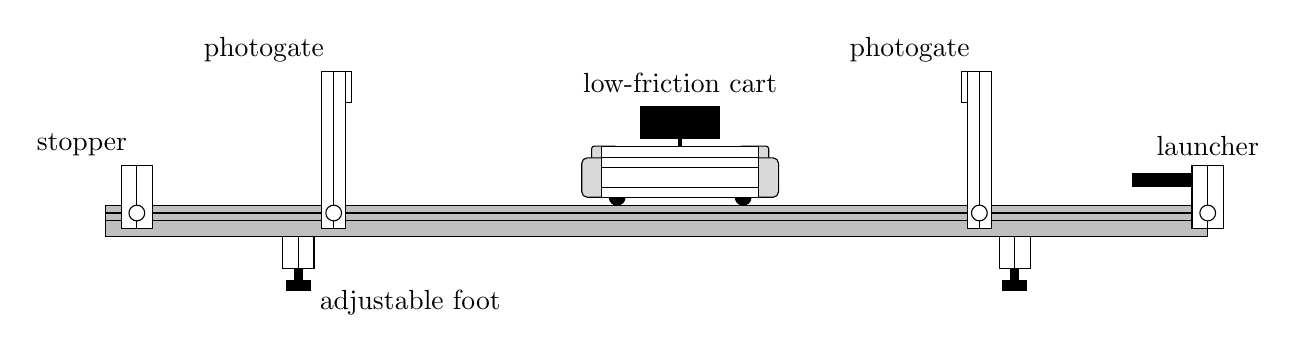
\begin{tikzpicture}
    \def\L{14}          % track length
    \def\t{0.2}         % track thickness
    \def\fx{2.25}       % foot distance from edge
    \def\fw{0.2}        % foot width
    \def\fh{0.4}        % foot height
    \def\sx{0.2}        % stopper distance from edge
    \def\sw{\fw}        % stopper width
    \def\sh{0.8}        % stopper height
    \def\soffset{0.1}   % stopper offset
    \def\pgx{2.75}      % photogate distance from edge
    \def\pgw{0.15}      % photogate width
    \def\pgh{2}         % photogate height
    \def\pgoffset{0.1}  % photogate offset
    \def\cw{2}          % cart width
    \def\ch{0.5}        % cart height
    \def\cx{0.45*\L}    % cart edge position
    \def\coffset{(2*\t+0.1)}   % cart offset from track
    % Draw the track bed
    \draw[fill=gray!50] (0,0) rectangle (\L,\t);
    \draw[fill=gray!50] (0,\t) rectangle (\L,{1.5*\t});
    \draw[fill=gray!50] (0,{1.5*\t}) rectangle (\L,{2*\t});
    % Draw the track feet
    \begin{scope}[shift={(\fx,-\fh)}]
        \draw[fill=white] (0,0) rectangle (\fw,\fh);
        \draw[fill=white] (\fw,0) rectangle ({2*\fw},\fh);
        \filldraw[black] (0.05,{-0.7*\fh}) rectangle ({2*\fw-0.05},{-0.4*\fh}) node[below right] {adjustable foot};
        \filldraw[black] ({0.75*\fw},{-0.4*\fh}) rectangle ({1.25*\fw},0);
    \end{scope}
    \begin{scope}[shift={({\L-\fx-2*\fw},-\fh)}]
        \draw[fill=white] (0,0) rectangle (\fw,\fh);
        \draw[fill=white] (\fw,0) rectangle ({2*\fw},\fh);
        \filldraw[black] (0.05,{-0.7*\fh}) rectangle ({2*\fw-0.05},{-0.4*\fh});
        \filldraw[black] ({0.75*\fw},{-0.4*\fh}) rectangle ({1.25*\fw},0);
    \end{scope}
    % Draw the stopper
    \draw[fill=white] (\sx,\soffset) rectangle ({\sx+\sw},{\soffset+\sh}) node[above left] {stopper};
    \draw[fill=white] ({\sx+\sw},\soffset) rectangle ({\sx+2*\sw},{\soffset+\sh});
    \draw[fill=white] ({\sx+\sw}, {3*\soffset}) circle (1mm);
    % Draw the cart and flag
    \begin{scope}[shift={(\cx,\coffset)}]
        \draw[fill=black] (0.2,0) circle (1mm);
        \draw[fill=black] ({\cw-0.2},0) circle (1mm);
        \draw[fill=gray!30, rounded corners=1] (-0.125,{\ch-0.15}) rectangle (0.2,{\ch+0.15});
        \draw[fill=gray!30, rounded corners=1] ({\cw-0.25},{\ch-0.15}) rectangle ({\cw+0.125},{\ch+0.15});
        \draw[fill=white] (0,\ch) rectangle (\cw,{\ch+0.15});
        \draw[fill=gray!30, rounded corners=2] (-0.25,0) rectangle (0.2,\ch);
        \draw[fill=gray!30, rounded corners=2] ({\cw-0.2},0) rectangle ({\cw+0.25},\ch);
        \draw[fill=white] (0,0) rectangle (\cw,\ch);
        \draw (0,{0.25*\ch}) -- (\cw,{0.25*\ch});
        \draw (0,{0.75*\ch}) -- (\cw,{0.75*\ch});
        \draw[ultra thick] ({0.5*\cw},{\ch+0.15}) -- ({0.5*\cw},{\ch+0.25});
        \filldraw[black] ({0.25*\cw},{\ch+0.25}) rectangle ({0.75*\cw},{\ch+0.65}) node[pos=0.5, yshift=5mm] {low-friction cart};
    \end{scope}
    % Draw the photogates
    \begin{scope}[shift={(\pgx,\pgoffset)}]
        \draw[fill=white] (0,0) rectangle (\pgw,\pgh) node[above left] {photogate};
        \draw[fill=white] (\pgw,0) rectangle ({2*\pgw},\pgh);
        \draw[fill=white] ({2*\pgw},\pgh) rectangle ({2*\pgw+0.075},{0.8*\pgh});
        \draw[fill=white] (\pgw,2*\pgoffset) circle (1mm);
    \end{scope}
    \begin{scope}[shift={(\L-\pgx-2*\pgw,\pgoffset)}]
        \draw[fill=white] (0,0) rectangle (\pgw,\pgh) node[above left] {photogate};
        \draw[fill=white] (\pgw,0) rectangle ({2*\pgw},\pgh);
        \draw[fill=white] (-0.075,\pgh) rectangle (0,{0.8*\pgh});
        \draw[fill=white] (\pgw,2*\pgoffset) circle (1mm);
    \end{scope}
    % Draw the spring launcher
    \begin{scope}[shift={(\L-\sw, 0)}]
        \filldraw[black] (-0.75,\sh) rectangle (0,{0.8*\sh});
        \draw[fill=white] (0,\soffset) rectangle (\sw,{\soffset+\sh}) node[above] {launcher};
        \draw[fill=white] (\sw,\soffset) rectangle ({2*\sw},{\soffset+\sh});
        \draw[fill=white] (\sw, {3*\soffset}) circle (1mm);
    \end{scope}
\end{tikzpicture}
        \caption{The linear track used in this experiment.}
        \label{fig: linear track}
    \end{figure}
    
    You will measure the velocity of the cart using a photogate, an electronic timer controlled by the interruption of an invisible infrared light beam. If an object of length $\ell$ interrupts the beam for a time interval $\Delta t$ while passing through the gate, then the average speed of the object during that time is given by
    %
    \begin{equation}
        v = \ell/\Delta t.
    \end{equation}
    %
    By measuring the velocity of the carts before and after various collisions, you will be able to calculate their energies and momenta to test the conservation laws.

    \subsection*{Notes on the Use and Setup of the Linear Track}

    \subsubsection*{Photogate Timers}

    Please note that although you usually use the two timers on the track at the same time, they work independently. In order to calculate the speed at a point on the track, use only the measurement from the timer at that position.

    \subsubsection*{Track}

    Several things must be done in preparation for experiments with the track. First, check if the track is level. Take one of the bubble levels provided for this purpose, place it lengthwise along the track above one of the supporting feet, and observe the position of the bubble. You want the bubble to be as close as possible to the middle of the level. To move the bubble, adjust the feet of the track by turning the screws at the base of the feet (see Fig.~\ref{fig: linear track}). When the bubble is centered in the level, repeat the procedure at the opposite end of the track with the level positioned lengthwise. Once both ends have been adjusted, repeat this again at both ends with the level along the width of the track.
    
    Second, make sure that there is an end stop at one end of the track and a launcher on the other end. To move the end stop and launcher, loosen the screws on the side and slide them into position (see Fig.~\ref{fig: cart and end stop}). Finally, align the two photogates so that they are about two and a half cart lengths apart.

    \begin{figure}[ht]
        \centering
        \fbox{
\includegraphics[height=4.25cm]{Lab 03: Conservation of Momentum/linear_track_cart.png}}
        % \hfill
        \fbox{
\includegraphics[height=4.25cm]{Lab 03: Conservation of Momentum/linear_track_stop.png}}
        \caption{Left: magnetic and velcro bumpers on the low-friction carts for testing elastic and inelastic collisions. Right: the stopper to be screwed into the end of the track. Image credits: PASCO Scientific.}
        \label{fig: cart and end stop}
    \end{figure}

    \subsubsection*{Cart}

    A description of the cart is given in Fig.~\ref{fig: cart and end stop}. One end of the cart has a magnet inside. The other end has a plunger and Velcro pads. You will use the magnetic bumpers for the elastic collisions and the Velcro for inelastic collisions. Note that the Velcro may not stick together well. To test this, push the plunger in all the way on both carts. Put the two carts together at their Velcro ends. If they are not sticking well, you can roughen the Velcro by repeatedly putting the carts together and pulling them apart, or by using the tape provided.

    Check that the carts have no irregularities by testing them on the track. Place each cart on the track, making sure that the wheels are in the grooves. Give each cart a small push and see how well it moves on the track. There should be minimal loss in speed as it rolls along the track. If there is a noticeable loss in speed, check the level of the track again. If the level is fine, check the wheels of the cart and then ask your TA for assistance.
    
    The track will be used to create various collisions between the carts. The collisions will be arranged so that an initially moving cart will pass through a photogate timer so you can measure its initial velocity. It will then hit the other cart, and one or both will pass through the photogate timers, allowing you to measure both final velocities. With these measured velocities, as well as the measured masses, the momentum and kinetic energy of the carts before and after the collisions can be calculated and compared.
    
    To reduce systematic uncertainties in this experiment, the approximate effects of friction will be measured, and launchers will be used so that the initial conditions of consecutive trials are reproducible.

    \subsection*{Newton's First Law}

    In this part of the experiment, one cart at a time will be rolled down the track past the two timers. The time for the cart to roll past each timer will be recorded.

    In the absence of friction, the cart's velocity should not change as it moves along the track, since no external forces would be acting on the cart. In reality, there will be a small amount of rolling friction present that reduces the cart's velocity. In this measurement, you will not be testing the conservation laws; you will take data to estimate the systematic uncertainty due to frictional losses. In the following sections, you will use the uncertainty to account for friction as you test the validity of the conservation laws.

    In the presence of friction, the ratios of the final to initial momentum (and energy) of the cart would be
    %
    \begin{align*}
        \frac{p_f}{p_i}&<1, & \frac{K_f}{K_i}&<1,
    \end{align*}
    %
    since small amounts of momentum and kinetic energy are lost as the cart rolls on the track. Here, you will measure the average final momentum $\overline{p}_f$ and the average final kinetic energy $\overline{K}_f$ of the cart, and use these to estimate the average fraction of momentum and kinetic energy lost due to friction:
    %
    \begin{align}
        \frac{\overline{\Delta p}}{p} &= 1 - \left(\frac{\overline{p}_f}{p_i}\right), \label{eq: average momentum loss}
        \\
        \frac{\overline{\Delta K}}{K} &= 1 - \left(\frac{\overline{K}_f}{K_i}\right). \label{eq: average energy loss}
    \end{align}

    \setlength{\fboxsep}{6pt}%
    \setlength{\fboxrule}{2pt}%
    \fbox{\begin{minipage}{0.9\textwidth}
        \color{RoyalBlue}
        {\bf Key Idea}: The average fractional losses give rough estimates of the amount of momentum and energy lost due to friction. If the average fractions lost when a collision occurs differ by \textbf{less than 3 times the average fractions lost} without a collision, then we will assume that no momentum or energy was lost in the collision, and therefore, that the conservation laws are valid since momentum and energy were only lost to friction.
    \end{minipage}}

    \subsubsection*{Procedure}

    \begin{enumerate}
        \item Answer question~\ref{q: friction loss estimate} in the Postlab exercises.

        \item Check that the track is level along both its length and width using the level provided (see instructions above). Test each direction at a few locations along the length of the track.

        \item Place a wooden block on top of one of the cars and stick a plastic board into the wood block so that it fits firmly. The plastic board is what the photogate timers will detect.

        \item Fix the heights of the photogates so that the board cuts the beam. A red LED indicator on the side of the photogate lights up when the beam is cut. You can adjust the height of the photogates by loosening the screw on the post and moving the bracket up or down. Make sure that you adjust both photogates and separate them by about 2.5 cart lengths.

        \item Adjust the cart launcher so that the scale reads around \qty{1}{\centi\meter} to \qty{2}{\centi\meter} when it is cocked. You can adjust the compression by loosening the screw on the latching clamp and sliding it into position.

        \item Take the cart you set up and place it in front of the launcher. Make sure the launcher is aimed at the center of the cart, and the cart's wheels are in the grooves of the track. \label{step: place cart}

        \item Launch the cart by pulling the string on the launcher. Once it has passed through both photogates, stop the cart and record the two photogate times in Data Table~\ref{data: fractional loss} in the Postlab exercises. \label{step: launch cart}

        \item Repeat steps \ref{step: place cart} and \ref{step: launch cart} again for a total of two trials.
    \end{enumerate}

    \subsection*{Elastic Collisions}

    In this part of the experiment, you will use two carts to create elastic collisions. Place two carts on the track with their magnetic ends facing each other and follow the procedure below. Some notes before you begin:

    \begin{itemize}
        \item The launcher setting and the positions of the timers are recommendations only. You are free to make any changes so long as they are consistent across all the trials.
        
        \item When positioning the timers, keep in mind that we want a measurement of the speed and direction of each of the two carts, both before and after the collisions.
        
        \item Remember that energy and momentum are lost continuously, mainly due to rolling friction, as the carts travel. Therefore, it is advisable to position the timers so that the measurements are taken just before and after the collision.
    \end{itemize}

    \noindent
    You will perform the following two experiments:
    %
    \begin{description}
        \item[Carts of equal mass]: Place the equal wooden masses on each cart. Set the launcher scale to around \qty{1}{\centi\meter} and separate the photogates by about 2.5 cart lengths.

        \item[Carts of unequal mass]: Place a wooden mass on the cart being launched and heavier, metal masses on the stationary cart. Set the launcher scale to around \qty{1}{\centi\meter}.
    \end{description}

    \subsubsection*{Procedure}

    \begin{enumerate}
        \item Answer question~\ref{q: elastic expected loss} in the Postlab exercises.

        \item Set up the launcher and photogates as described in the instructions for \textbf{Carts of equal mass}.

        \item Launch one of the carts into the other (stationary) one. Set it up so that the collision occurs between the photogate timers. The launched cart should pass through the first timer before the collision, and this time should be recorded in Data Table~\ref{data: elastic collision} as $t_{1,i}$. The final times of both carts can be read off the photogate timers after the collision and entered in Data Table~\ref{data: elastic collision} as well.

        \item Both timers should be set to gate mode. If one of the timers reads two times, then the individual times need to be found. The displayed time is the first time, $t_1$. To get the second time, $t_1$, flip the memory switch to get the total time, $t_1+t_2$, and subtract the first time from this to get the second time, $t_2$.

        \item Replace the wooden mass on the stationary cart with a metal mass so that $m_1<m_2$. If the wooden cart derails after the collision, turn down the launcher power until it no longer derails. You will not need to take time measurements, but qualitatively observe the behavior of this collision and answer question~\ref{q: elastic unequal masses} in the Postlab exercises.
    \end{enumerate}

    \subsection*{Inelastic Collisions}

    In an inelastic collision, the two carts should stick together after the collision, so you should have the Velcro ends of the carts facing each other. We will be using the same setup as before, with one cart with mass $m_1$ in front of the launcher and one cart with mass $m_2$ at rest on the track. Our goal is to find which combination of masses causes the least kinetic energy to be lost in the collision. 

    \subsubsection*{Procedure}

    \begin{enumerate}
        \item Set $m_1<m_2$ by adding the wooden mass to the cart next to the launcher and the metal mass to the cart between the photogates. Set the launcher scale to \qty{2}{\centi\meter}.

        \item Place the carts onto the track so that the Velcro ends face each other. If the carts do not stick together after the collision, add tape to the end of the stationary cart to increase its stickiness.

        \item Launch the cart and observe the time $t_1$ of the first cart and the time $t_2$ of the two-cart system. Record your results in Data Table~\ref{data: inelastic collision} in the Postlab exercises. \label{step: inelastic launch}

        \item Repeat your measurement so that you have two trials and record your results in Data Table~\ref{data: inelastic collision} in the Postlab exercises. \label{step: inelastic record}

        \item Set up the carts to have equal mass ($m_1=m_2$) and repeat steps \ref{step: inelastic launch} and \ref{step: inelastic record}.

        \item Set up the carts so that the stationary cart has less mass than the moving cart ($m_1>m_2$) and repeat steps \ref{step: inelastic launch} and \ref{step: inelastic record}.
    \end{enumerate}   

    \subsection*{Velocity of a Projectile using a Ballistic Pendulum}

    In this part of the lab, you will measure the velocity of a projectile using a ballistic pendulum (see Fig.~\ref{fig: ballistic pendulum}). The projectile will be a metal ball launched with a spring gun.\\[1em]

    \setlength{\fboxsep}{6pt}%
    \setlength{\fboxrule}{2pt}%
    \fbox{\begin{minipage}{0.9\textwidth}
        \color{RubineRed}
        {\bf CAUTION}: Never look into the barrel of the launcher or put your fingers into the barrel!
    \end{minipage}}

    \subsubsection*{Procedure}

    \begin{enumerate}
        \item Make sure the base of the ballistic pendulum apparatus is level and adjust it if necessary.

        \item Measure the mass $m$ of the metal ball and record it in Data Table~\ref{data: ballistic pendulum} in the Postlab exercises.
        
        \item The ball mounts on the spring gun's push rod via a hole through its diameter. Ensure that the projectile loads smoothly on your apparatus, and that the ball catcher at the pendulum is aligned with the barrel of the spring gun.
        
        \item Measure the mass $M$ of the pendulum and ball catcher by carefully unscrewing the pivot pin, which is the small knob at the top of the pendulum. Slide out the pin and remove the pendulum. Place the pin in a safe place so that it is not lost while you weigh the pendulum. Record the pendulum + ball catcher mass in Data Table~\ref{data: ballistic pendulum} in the Postlab exercises. \label{step: pendulum mass}
        
        \item Find the distance $R$ from the pivot pin to the center-of-mass of the ball-pendulum system. Place the metal ball in the catcher and balance the entire assembly on the edge of the table.
        %
        \begin{center}
            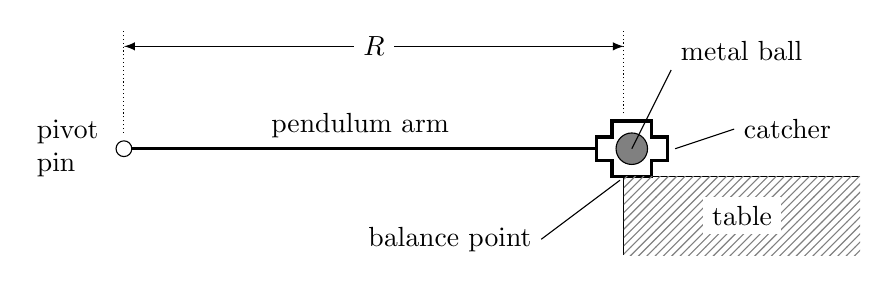
\begin{tikzpicture}
    % Pendulum pivot pin and arm
    \draw[very thick] (0,0) -- node[midway, above] {pendulum arm} (6,0);
    \draw[fill=white] (0,0) circle (1mm) node[left, align=left, xshift=-2mm] {pivot\\pin};
    % Draw the mass and the catcher
    \draw[very thick] (6,-0.15) -- ++(0,0.3) -- ++(0.2,0) -- ++(0,0.2) -- ++(0.5,0) -- ++(0,-0.2) -- ++(0.2,0) -- ++(0,-0.3) -- ++(-0.2,0) -- ++(0,-0.2) -- ++(-0.5,0) -- ++(0,0.2) -- cycle;
    \draw[fill=gray] (6.45,0) circle (2mm);
    \draw (6.45,0) -- ++(0.5,1) node[above right] {metal ball};
    \draw (7,0) -- ++(0.75,0.25) node[right] {catcher};
    % Table
    \draw (6.35,-1.35) -- ++(0,1) -- ++(3,0);
    \fill[pattern color=gray, pattern={north east lines}] (6.35,-1.35) rectangle ++(3,1) node[pos=0.5, fill=white] {table};
    \draw ((6.3,-0.4) -- ++(-1,-0.75) node[left] {balance point};
    % Mark the distance R
    \draw[densely dotted] (0,0.2) -- (0,1.5);
    \draw[densely dotted] (6.35,0.45) -- (6.35,1.5);
    \draw[latex-latex] (0,1.3) -- node[midway,fill=white] {$R$} (6.35,1.3);
\end{tikzpicture}
            \captionsetup{font=normalsize}
            \captionof{figure}{Finding the center of mass of the pendulum + ball by balancing it on the table edge. \label{fig: balance pendulum}}
        \end{center}
        %
        As shown in Fig~\ref{fig: balance pendulum}, move it until the assembly is just barely balanced, and moving it any farther out would cause it to fall over. The balance point will be directly under the center of mass of the assembly. Measure $R$ as the distance between the pivot pin and the center of mass, and record your value in Data Table~\ref{data: ballistic pendulum} in the Postlab exercises.
        
        \item Replace the pendulum by reversing the disassembly sequence in step~\ref{step: pendulum mass}.

        \item Cock the gun by placing the ball in the launcher’s barrel. Then push the ball down the barrel with the ramrod until the trigger catches the piston at the desired point.
        
        \item There are three range settings: short, medium, and long. We recommend using the long-range setting, but feel free to use any of them, as long as you use the same setting for each trial.

        \item Starting with the pendulum at rest and the angle indicator set to zero, fire the ball into the catcher five times and measure the maximum angle to which the pendulum
        swings each time. Make sure the spring gun is at the same setting for each trial and record your data in Data Table~\ref{data: ballistic pendulum}.
        
        \textbf{Be careful not to get your hand caught in the spring gun}.
    \end{enumerate}

    \subsection*{Velocity of a Projectile using a Projectile Motion}

    In the final part of the lab, you will measure the velocity of a projectile by launching it from the same spring gun used with the ballistic pendulum, as shown in Fig.~\ref{fig: projectile motion}. By observing the projectile's motion, you can use the equations of kinematics to infer its initial velocity.

    \subsubsection*{Procedure}

    \begin{enumerate}
        \item Make sure that the apparatus is securely fastened and leveled on a block on the table. Latch the pendulum bob out of the way and practice firing the ball from the gun out onto the floor. Be careful of wild shots.

        \item Measure the height, $H$, from the floor to the bottom of the ball when it is sitting in the launcher. (It is simplest to measure the distance between the floor and the table top, and the table top to the bottom of the ball, and add the two values.) Record it in \textbf{Table Z} of the Postlab exercises.

        \item With the ball in the gun and the spring uncompressed, so the ball sits at the front of the cannon, find the position on the table directly below the center of the ball and mark it with a piece of tape.

        \item With the ball in place, compress the spring to whatever range you prefer and then pull up on the string to release the spring and launch the ball. Tape a piece of white paper over the area where the ball landed and cover it with carbon paper, carbon side down. Do not tape the carbon paper!

        \item Reload the spring gun and fire the ball five more times using the same range setting. The ball should leave carbon marks on the paper so that you can measure the horizontal distance the ball traveled. Record each distance, $L$, in \textbf{Table Z}.
    \end{enumerate}
    
\end{experiment}

\end{labsection}

% Postlab questions
\begin{postlab}

    \fullwidth{\subsection*{Newton's First Law (\pointsinrange{newtons1st} points)}}

    \begingradingrange{newtons1st}

    \filbreak
    \question \label{q: friction loss estimate}
    \begin{parts}
        \part[\half] What values do you expect for the fractions of momentum and kinetic energy lost,
        %
        \begin{align*}
            \frac{\Delta p}{p} &= ?
            &
            \frac{\Delta K}{K} &= ?
        \end{align*}
        %
        when friction is infinitely large? Why?
        \begin{solution}[1.25cm]
        \end{solution}

        \part[\half] What about when there is no friction? Why?
        \begin{solution}[1.25cm]
        \end{solution}
    \end{parts}

    \filbreak
    \question[1]\label{q: fraction lost newton}
    Fill in Data Table~\ref{data: fractional loss}, where $t_i$ is the time in the first photogate and $t_f$ is the time in the second photogate.
    %
    \begin{center}
        \captionsetup{font=normalsize}
        \captionof{data table}{Measurements of fractional energy and momentum loss. \label{data: fractional loss}}
        \renewcommand{\arraystretch}{2}
        \begin{tabular}{|>{\centering\arraybackslash}p{1.5cm}|>{\centering\arraybackslash}p{2cm}|>{\centering\arraybackslash}p{2cm}|>{\centering\arraybackslash}p{2cm}|>{\centering\arraybackslash}p{2cm}|}
        \hline
        \rowcolor{gray!20}
        Trial & $t_i$ & $t_f$ & $p_f/p_i$ & $K_f/K_i$
        \\
        \hline
        1 & & & & \\ \hline
        2 & & & & \\ \hline
        \end{tabular}
    \end{center}
    %
    Note that if the cart has length $\ell$, its velocity at each photogate is $v_i=\ell/t_i$ and $v_f=\ell/t_f$. Thus, the momentum and energy fractions are
    %
    \begin{align*}
        \frac{p_f}{p_i} &= \frac{mv_f}{mv_i} = \frac{m(\ell/t_f)}{m(\ell/t_i)} = \frac{t_i}{t_f},
        &
        \frac{K_f}{K_i} &= \frac{\nicefrac{1}{2}~mv_f^2}{\nicefrac{1}{2}~mv_i^2} = \frac{\nicefrac{1}{2}~m(\ell/t_f)^2}{\nicefrac{1}{2}~m(\ell/t_i)^2} = \frac{t_i^2}{t_f^2}.
    \end{align*}
    %
    Compute the average fractions conserved and calculate the fractions lost with eqs.~\ref{eq: average momentum loss} and \ref{eq: average energy loss}. Show your work.

    \begin{align*}
        \frac{\overline{\Delta p}}{p} &= \qquad\qquad\qquad\qquad\qquad\qquad\qquad\qquad\qquad
        &
        \frac{\overline{\Delta K}}{K} &= \qquad\qquad\qquad\qquad\qquad\qquad\qquad\qquad\qquad
    \end{align*}

    \endgradingrange{newtons1st}

    %%% Elastic collisions
    \newpage
    \fullwidth{\subsection*{Elastic Collisions of Equal and Unequal Masses (\pointsinrange{elastic} points)}}

    \begingradingrange{elastic}

    \filbreak
    \question \label{q: elastic expected loss}
    \begin{parts}
        \part[\half] For a perfectly elastic collision, what values do you expect for the fractions lost given the effect of friction that you measured?
        %
        \begin{align*}
            \frac{\overline{\Delta p}}{p} &= \qquad\qquad\qquad\qquad\qquad\qquad\qquad\qquad\qquad
            &
            \frac{\overline{\Delta K}}{K} &= \qquad\qquad\qquad\qquad\qquad\qquad\qquad\qquad\qquad
            \\
        \end{align*}

        \part[\half] Why do you think these values would be the same or different than the ones you calculated in question \ref{q: fraction lost newton}?
        \begin{solution}[2cm]
        \end{solution}
    \end{parts}

    \filbreak
    \question \label{q: fraction lost equal mass}
    \begin{parts}
        \part[\half] If we assume the lengths and masses of the two carts are equal, will the simplified equations for the fractions conserved that you used before still hold? Why?
        \begin{solution}[2cm]
            
        \end{solution}

        \part[\half] Based on your answer to part (a), what equation (simplified or not) will you use to compute $\overline{\Delta p}/p$ and $\overline{\Delta K}/K$, the fractions lost?
        \begin{solution}[2cm]
            
        \end{solution}
    \end{parts}

    \filbreak
    \question[1] Fill in Data Table~\ref{data: elastic collision}. The launched cart is mass $m_1$ and the stationary cart is mass $m_2$; $t_{1,i}$ is the time $m_1$ passes the first photogate before the collision, and $t_{2,f}$ is the time the second cart passes the second photogate after the collision.
    %
    \begin{center}
        \captionsetup{font=normalsize}
        \captionof{data table}{Measurements of elastic collisions between equal masses. \label{data: elastic collision}}
        \renewcommand{\arraystretch}{2}
        \begin{tabular}{|>{\centering\arraybackslash}p{1.5cm}|>{\centering\arraybackslash}p{1.5cm}|>{\centering\arraybackslash}p{1.5cm}|>{\centering\arraybackslash}p{1.5cm}|>{\centering\arraybackslash}p{1.5cm}|>{\centering\arraybackslash}p{1.5cm}|>{\centering\arraybackslash}p{1.5cm}|}
        \hline
        \rowcolor{gray!20}
        Trial & $m_1$ & $m_2$ & $t_{1,i}$ & $t_{1,f}$ & $t_{2,i}$ & $t_{2,f}$
        \\
        \hline
        1 & & & & N/A & N/A & \\ \hline
        \end{tabular}
    \end{center}
    %
    \begin{solution}[1cm]
            
    \end{solution}

    \filbreak
    \question[1] \label{q: fraction lost elastic} Using your answer to question~\ref{q: fraction lost equal mass} and the data in Data Table~\ref{data: elastic collision}, find the fractions of momentum and kinetic knergy lost. 
    %
    \begin{align*}
        \frac{\overline{\Delta p}}{p} &= \qquad\qquad\qquad\qquad\qquad\qquad\qquad\qquad\qquad
        &
        \frac{\overline{\Delta K}}{K} &= \qquad\qquad\qquad\qquad\qquad\qquad\qquad\qquad\qquad
        \\
    \end{align*}
    %
    \begin{solution}[1cm]
            
    \end{solution}

    \filbreak
    \question[1] Following the key idea in the discussion of fractional energy loss, determine if the following inequalities are satisfied:
    %
    \begin{equation}
        \left|\left(\frac{\overline{\Delta p}}{p}\right)_\text{Question \ref{q: fraction lost elastic}} - \left(\frac{\overline{\Delta p}}{p}\right)_\text{Question \ref{q: fraction lost newton}}\right| > 3\left(\frac{\overline{\Delta p}}{p}\right)_\text{Question \ref{q: fraction lost newton}},
    \end{equation}
    %
    and
    %
    \begin{equation}
        \left|\left(\frac{\overline{\Delta K}}{K}\right)_\text{Question \ref{q: fraction lost elastic}} - \left(\frac{\overline{\Delta K}}{K}\right)_\text{Question \ref{q: fraction lost newton}}\right| > 3\left(\frac{\overline{\Delta K}}{K}\right)_\text{Question \ref{q: fraction lost newton}}.
    \end{equation}
    %
    In other words, is the fractional change in momentum and energy during the collision at least 3 times larger than the losses due to friction?
    %
    \begin{solution}[3cm]
        
    \end{solution}

    \filbreak
    \question[1] \label{q: elastic unequal masses} After you replace the wooden block with a metal weight in the stationary mass, such that $m_1<m_2$, observe the collision and describe what you observe. Think about what happens in this collision, and how it is different from the equal mass collision. Look back at the simplified equations for the fractions conserved; do they still apply in this case?
    %
    \begin{solution}[5cm]
        
    \end{solution}

    \endgradingrange{elastic}

    % Inelastic collisions
    \newpage
    \fullwidth{\subsection*{Inelastic Collisions (\pointsinrange{inelastic} points)}}

    \begingradingrange{inelastic}
    
    \filbreak
    \question[1] Measure the inelastic collision by launching a cart into a stationary cart. Record your data for three different mass combinations in Data Table~\ref{data: inelastic collision}.
    %
    \begin{center}
        \captionsetup{font=normalsize}
        \captionof{data table}{Measurements of inelastic collisions between masses. \label{data: inelastic collision}}
        \renewcommand{\arraystretch}{2}
        \begin{tabular}{|>{\centering\arraybackslash}p{2cm}|>{\centering\arraybackslash}p{2cm}|>{\centering\arraybackslash}p{2cm}|}
            \hline
            \rowcolor{gray!20}
            Trial & $t_1$ & $t_2$ \\ \hline
            \multirow{2}{*}{$m_1<m_2$} & & \\ \cline{2-3}
            & & \\ \hline 
            \multirow{2}{*}{$m_1=m_2$} & & \\ \cline{2-3}
            & & \\ \hline 
            \multirow{2}{*}{$m_1>m_2$} & & \\ \cline{2-3}
            & & \\ \hline 
        \end{tabular}
    \end{center}
    %
    \begin{solution}[1cm]
        
    \end{solution}

    \filbreak
    \question
    \begin{parts}
        \part[\half] Which of the combinations that you tested ($m_1<m_2$; $m_1=m_2$; and $m_1>m_2$) led to the smallest change in speed of the two carts after the collision?
        %
        \begin{solution}[1cm]
            
        \end{solution}

        \part[\half] Why do you think that this combination worked best? Remember from eq.~\ref{eq: inelastic collision final velocity} that for an inelastic collision, momentum conservation tells us
        \[
            m_1u_1 = (m_1+m_2)v.
        \]
        \begin{solution}[2cm]
            
        \end{solution}
    \end{parts}

    \filbreak
    \question[1] What is one factor that limits the final velocity $v$ of the two carts?
    %
    \begin{solution}[1cm]
        
    \end{solution}

    \endgradingrange{inelastic}

    %%% Ballistic pendulum
    \newpage
    \fullwidth{\subsection*{Velocity Measurements with a Ballistic Pendulum (\pointsinrange{ballistic} points)}}
    
    \begingradingrange{ballistic}

    \filbreak
    \question[1] Fill in measurements from the ballistic pendulum in Data Table~\ref{data: ballistic pendulum}
    %
    \begin{center}
        \captionsetup{font=normalsize}
        \captionof{data table}{Measurements of the ballistic pendulum. \label{data: ballistic pendulum}}
        \renewcommand{\arraystretch}{2}
        \begin{tabular}{|g|>{\centering\arraybackslash}p{1.5cm}|>{\centering\arraybackslash}p{1.5cm}|>{\centering\arraybackslash}p{1.5cm}|>{\centering\arraybackslash}p{1.5cm}|>{\centering\arraybackslash}p{1.5cm}|>{\centering\arraybackslash}p{1.5cm}|}
            \multicolumn{1}{r}{$R=$} & \multicolumn{2}{c}{} & \multicolumn{4}{c}{} \\ \cline{2-3}
            \multicolumn{1}{r}{Ball mass $m=$} & \multicolumn{2}{c}{} & \multicolumn{4}{c}{} \\ \cline{2-3}
            \multicolumn{1}{r}{Pendulum mass $M=$} & \multicolumn{2}{c}{} & \multicolumn{4}{c}{} \\ \cline{2-3}
            \multicolumn{7}{c}{} \\
            \hline
            \rowcolor{gray!20}
            Trial & 1 & 2 & 3 & 4 & 5 & $\overline{h}$ \\ \hline
            Angle $\theta$ & & & & & & --- \\ \hline
            $h=R(1-\cos{\theta})$ & & & & & & \\ \hline
        \end{tabular}
    \end{center}
    %
    \begin{solution}[1cm]
        
    \end{solution}

    \filbreak
    \question[1] Calculate the average height of the center of mass of the ball, $h$, and its standard deviation, $\Delta h$. Show your work, including units.
    %
    \begin{solution}[3cm]
        
    \end{solution}

    \filbreak
    \question[1] \label{q: ballistic velocity} Using the results of the calculation above, find the initial velocity of the ball, $v_b$, using eq.~\ref{eq: ballistic pendulum vi}, where $v_b=u$. Show your work and include units with your answer.
    %
    \begin{solution}[3cm]
        
    \end{solution}

    \filbreak
    \question[1] \label{q: ballistic uncertainty} Find the uncertainty in the ball's velocity, $\Delta v_b$, using propagation of uncertainties:
    \[
        \frac{\Delta v_b}{v_b} = \frac{\Delta h}{2\overline{h}}.
    \]
    Note that we assume the measurement of mass has no uncertainty. Show your work.
    %
    \begin{solution}[3cm]
        
    \end{solution}
    
    \endgradingrange{ballistic}

    %%% Projectile motion
    \newpage
    \fullwidth{\subsection*{Velocity Measurements from Projectile Motion (\pointsinrange{projectile} points)}}
    
    \begingradingrange{projectile}

    \filbreak
    \question[1] Record your measurement of $H$, its estimated uncertainty $\Delta H$, and all of the range measurements $L$ in Data Table~\ref{data: projectile motion}. 
    %
    \begin{center}
        \captionsetup{font=normalsize}
        \captionof{data table}{Measurements of projectile motion. \label{data: projectile motion}}
        \renewcommand{\arraystretch}{2}
        \begin{tabular}{|g|>{\centering\arraybackslash}p{1.5cm}|>{\centering\arraybackslash}p{1.5cm}|>{\centering\arraybackslash}p{1.5cm}|>{\centering\arraybackslash}p{1.5cm}|>{\centering\arraybackslash}p{1.5cm}|c|}
            \multicolumn{1}{r}{$H=$} & \multicolumn{2}{c}{} & \multicolumn{4}{c}{} \\ \cline{2-3}
            \multicolumn{1}{r}{$\Delta H=$} & \multicolumn{2}{c}{} & \multicolumn{4}{c}{} \\ \cline{2-3}
            \multicolumn{7}{c}{} \\
            \hline
            \rowcolor{gray!20}
            Trial & 1 & 2 & 3 & 4 & 5 & Average $\overline{L}$ \\ \hline
            Distance $L$ & & & & & & \\ \hline
        \end{tabular}
    \end{center}
    %
    \begin{solution}[1cm]
        
    \end{solution}

    \filbreak
    \question[1] Calculate the average range that the ball travels, $\overline{L}$ and its uncertainty $\Delta L$ (i.e. the standard deviation of your measurements). Show your work.
    %
    \begin{solution}[4cm]
        
    \end{solution}

    \filbreak
    \question[1] Calculate $v_b$ from your measurements of $H$ and $\overline{L}$ using eq.~\ref{eq: projectile velocity}. Show your work.
    %
    \begin{solution}[3cm]
        
    \end{solution}


    \filbreak
    \question[1] Calculate the uncertainty in the initial velocity, $\Delta v_b$, using propagation of uncertainties:
    \[
        \frac{\Delta v_b}{v_b} = \sqrt{\left(\frac{\Delta L}{\overline{L}}\right)^2 + \left(\frac{\Delta H}{2H}\right)^2}.
    \]
    Show your work, and include correct units in your answer.
    %
    \begin{solution}[5cm]
        
    \end{solution}

    \filbreak
    \question
    \begin{parts}
        \part[\half] Is the initial velocity of the ball $v_b$ and its uncertainty $\Delta v_b$ calculated with projectile motion consistent with the values calculated using the ballistic pendulum and conservation laws (questions \ref{q: ballistic velocity} and \ref{q: ballistic uncertainty})? I.e., do the results agree within uncertainties? 
        %
        \begin{solution}[2cm]
            
        \end{solution}

        \part[\half] If the measurements do not agree, what is one factor that could have caused this discrepancy?
        %
        \begin{solution}[2cm]
            
        \end{solution}
    \end{parts}
    
    \endgradingrange{projectile}

\end{postlab}

\end{document}